% Generated by hackathon_agents.tools.adc_study_paper
\documentclass[10pt]{article}
\usepackage[T1]{fontenc}
\usepackage{longtable}
\usepackage[utf8]{inputenc}
\usepackage[margin=0.7in]{geometry}
\usepackage{graphicx}
\usepackage{booktabs}
\usepackage{amsmath}
\usepackage{amssymb}
\usepackage{array}
\usepackage{caption}
\captionsetup{font=small}
\usepackage[hidelinks]{hyperref}
\usepackage{titlesec}
\titleformat*{\section}{\large\bfseries}
\titleformat*{\subsection}{\normalsize\bfseries}
\setlength{\parskip}{0.15em}
\graphicspath{{./}{figures/}}
\title{\textbf{Supplementary Information: Payload-Aware Autonomous ADC Linker Design}}
\author{Elia Savino$^{1,d}$, Joshua W.\ Sin$^{2,3,d}$, Morgan G.\ L.\ Reigner$^{1,d}$, Miqu\`el \`A.\ P\'erez-Puigdom\`enech$^{2,d}$, Derk H.\ W.\ ten Klooster$^{1,d}$, Claude$^{d}$, J.A.R.V.I.S$^{d}$}
\date{}
\begin{document}
\maketitle
\section{Full context ranking (all 38 contexts)}
\begin{longtable}{l l l c c c c}\toprule
Handle & Trigger & Payload & mean & best & SD & seeds \\ \midrule\endhead
Oxyamine & Non-cleavable & cytotoxin & 0.92 & 0.93 & 0.01 & 2 \\
Tetrazine & Non-cleavable & cytotoxin & 0.90 & 0.91 & 0.02 & 2 \\
Bromoacetamide & Non-cleavable & cytotoxin & 0.85 & 0.87 & 0.01 & 2 \\
DBCO & Non-cleavable & immunomodulator & 0.78 & 0.82 & 0.04 & 2 \\
NHS\_ester & Non-cleavable & cytotoxin & 0.82 & 0.82 & 0.00 & 2 \\
DBCO & Non-cleavable & cytotoxin & 0.76 & 0.81 & 0.05 & 2 \\
DBCO & Non-cleavable-rigid & immunomodulator & 0.79 & 0.80 & 0.01 & 2 \\
DBCO & Non-cleavable & oligonucleotide & 0.79 & 0.80 & 0.01 & 2 \\
DBCO & Non-cleavable-rigid & cytotoxin & 0.78 & 0.78 & 0.01 & 2 \\
DBCO & Non-cleavable-rigid & oligonucleotide & 0.75 & 0.76 & 0.01 & 2 \\
Maleimide & Non-cleavable & cytotoxin & 0.72 & 0.75 & 0.02 & 2 \\
Maleimide & Non-cleavable & immunomodulator & 0.72 & 0.74 & 0.02 & 2 \\
TCO & Non-cleavable & cytotoxin & 0.68 & 0.70 & 0.02 & 2 \\
Maleimide & Non-cleavable-rigid & oligonucleotide & 0.68 & 0.68 & 0.00 & 2 \\
Maleimide & Non-cleavable & oligonucleotide & 0.67 & 0.68 & 0.01 & 2 \\
Maleimide & Non-cleavable-rigid & immunomodulator & 0.67 & 0.68 & 0.00 & 2 \\
Maleimide & Non-cleavable-rigid & cytotoxin & 0.67 & 0.67 & 0.00 & 2 \\
Tetrazine & Val-Cit-PABC & cytotoxin & 0.59 & 0.61 & 0.03 & 2 \\
Bromoacetamide & Val-Cit-PABC & cytotoxin & 0.58 & 0.60 & 0.02 & 2 \\
Oxyamine & Val-Cit-PABC & cytotoxin & 0.59 & 0.60 & 0.01 & 2 \\
NHS\_ester & Val-Cit-PABC & cytotoxin & 0.58 & 0.59 & 0.01 & 2 \\
Disulfide & Non-cleavable & cytotoxin & 0.57 & 0.59 & 0.02 & 2 \\
TCO & Val-Cit-PABC & cytotoxin & 0.56 & 0.56 & 0.00 & 2 \\
DBCO & Val-Cit-PABC & immunomodulator & 0.53 & 0.55 & 0.02 & 2 \\
DBCO & Val-Cit-PABC & cytotoxin & 0.51 & 0.53 & 0.02 & 2 \\
Maleimide & Val-Cit-PABC & immunomodulator & 0.52 & 0.52 & 0.00 & 2 \\
Maleimide & Val-Cit-PABC & cytotoxin & 0.51 & 0.51 & 0.00 & 2 \\
Disulfide & Val-Cit-PABC & cytotoxin & 0.42 & 0.43 & 0.02 & 2 \\
DBCO & Val-Cit-PABC & oligonucleotide & 0.38 & 0.40 & 0.02 & 2 \\
Maleimide & Val-Cit-PABC & oligonucleotide & 0.35 & 0.36 & 0.01 & 2 \\
Maleimide & Glucuronide & cytotoxin & 0.08 & 0.08 & 0.00 & 2 \\
Bromoacetamide & Glucuronide & cytotoxin & 0.08 & 0.08 & 0.00 & 2 \\
Oxyamine & Glucuronide & cytotoxin & 0.08 & 0.08 & 0.00 & 2 \\
NHS\_ester & Glucuronide & cytotoxin & 0.08 & 0.08 & 0.00 & 2 \\
Tetrazine & Glucuronide & cytotoxin & 0.08 & 0.08 & 0.00 & 2 \\
DBCO & Glucuronide & cytotoxin & 0.08 & 0.08 & 0.00 & 2 \\
TCO & Glucuronide & cytotoxin & 0.08 & 0.08 & 0.00 & 2 \\
Disulfide & Glucuronide & cytotoxin & 0.07 & 0.07 & 0.00 & 2 \\
\bottomrule\end{longtable}
\begin{figure}[t]\centering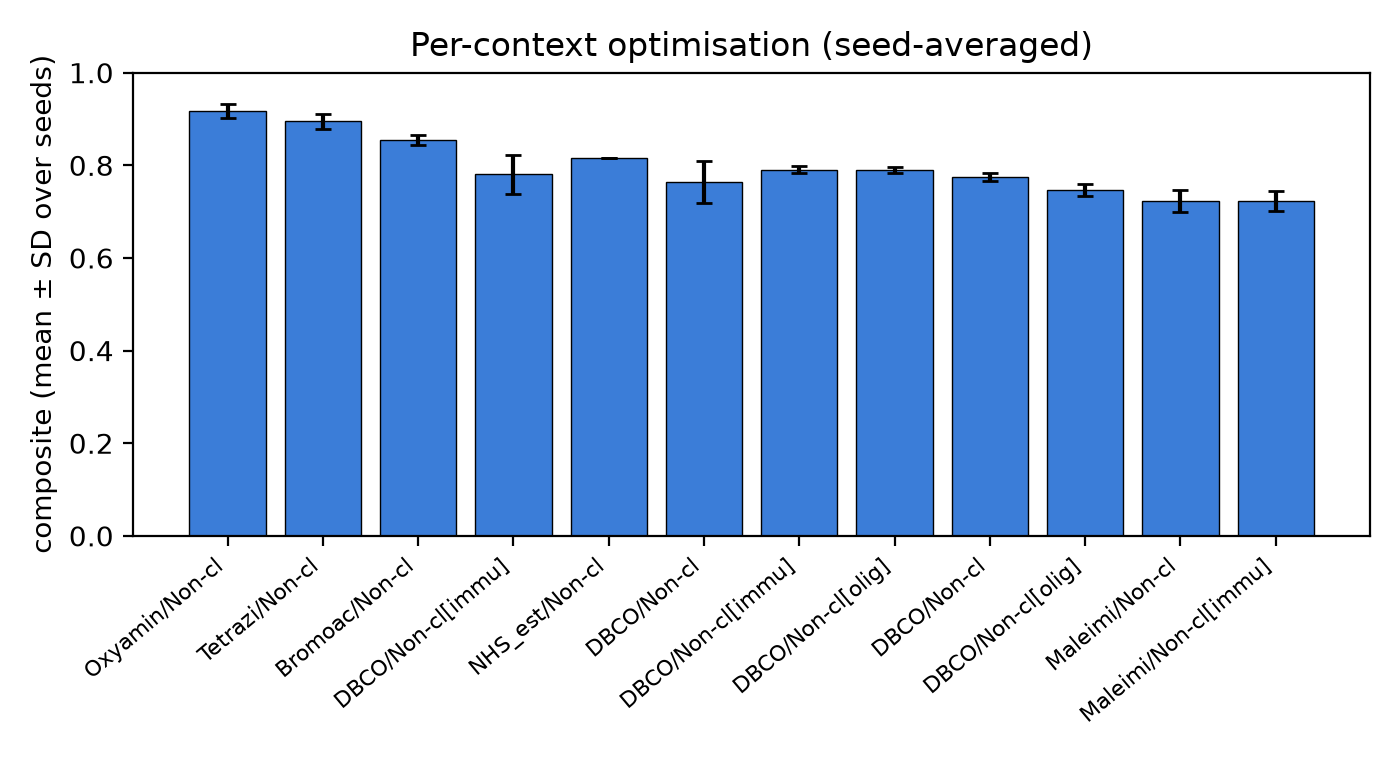
\includegraphics[width=0.9\linewidth]{fig_context_bars.png}\caption{Per-context optimisation, mean $\pm$ SD over seeds (top contexts). Modest seed variance supports the ranking.}\label{fig:sbars}\end{figure}
\section{Payload-class re-scoring (mean composite by payload rule)}
\begin{longtable}{l l c c c}\toprule
Handle & Trigger & cytotoxin & oligonucleotide & immunomodulator \\ \midrule\endhead
DBCO & Non-cleavable & 0.76 & 0.79 & 0.78 \\
DBCO & Non-cleavable-rigid & 0.78 & 0.75 & 0.79 \\
Maleimide & Non-cleavable & 0.72 & 0.67 & 0.72 \\
Maleimide & Non-cleavable-rigid & 0.67 & 0.68 & 0.67 \\
DBCO & Val-Cit-PABC & 0.51 & 0.38 & 0.53 \\
Maleimide & Val-Cit-PABC & 0.51 & 0.35 & 0.52 \\
\bottomrule\end{longtable}
\begin{figure}[t]\centering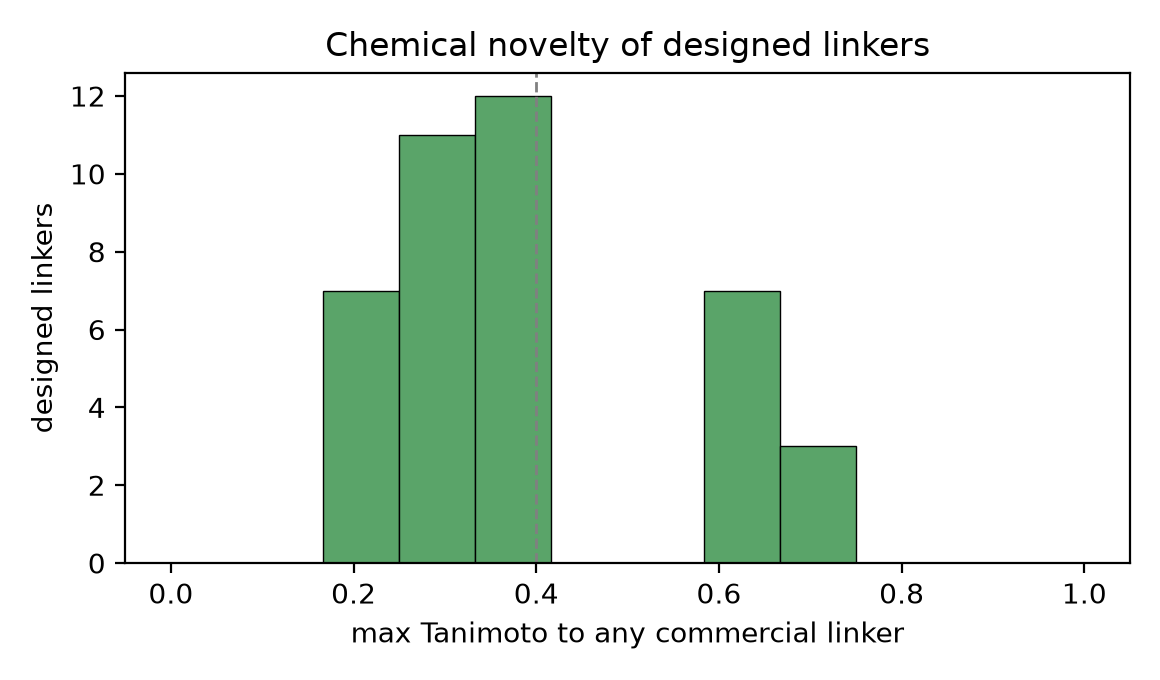
\includegraphics[width=0.7\linewidth]{fig_novelty.png}\caption{Chemical novelty: nearest-neighbour Tanimoto of each designed linker to any commercial linker. Most designs are distinct chemotypes (similarity $<0.4$), not rediscoveries.}\label{fig:snov}\end{figure}
\section{Table S1: Stability-surrogate calibration}
\begin{tabular}{l c l}\toprule
Mechanistic class & stability & expected \\ \midrule
acid-labile hydrazone & 0.00 & low \\
redox disulfide & 0.80 & intermediate \\
protease dipeptide & 0.85 & high \\
non-cleavable thioether & 0.85 & high \\
\bottomrule\end{tabular}\par\smallskip
\section{Commercial linker benchmark}
\begin{longtable}{l l c c c}\toprule
Name & ADC / class & composite & QED & MW \\ \midrule\endhead
mc-Val-Cit-PABC & brentuximab vedotin (Ad... & 0.37 & 0.116 & 573 \\
mc-Val-Ala-PABC & Val-Ala class & 0.40 & 0.244 & 487 \\
mc-GGFG & trastuzumab deruxtecan ... & 0.39 & 0.128 & 530 \\
MCC (non-cleavable) & trastuzumab emtansine (... & 0.59 & 0.737 & 237 \\
SPDB disulfide & mirvetuximab soravtansi... & 0.62 & 0.600 & 229 \\
sulfo-SPDB & hindered disulfide class & 0.66 & 0.444 & 309 \\
AcBut hydrazone & gemtuzumab ozogamicin (... & 0.00 & 0.340 & 236 \\
beta-glucuronide & glucuronide linker class & 0.00 & 0.156 & 508 \\
maleimidocaproyl (mc) & mc handle & 0.59 & 0.514 & 211 \\
\bottomrule\end{longtable}
\section{Table S2: Top designed linkers (full SMILES)}
\begin{longtable}{l l c p{9cm}}\toprule
Context & Payload & Score & SMILES \\ \midrule\endhead
Oxyami/Non-cl & cytot & 0.93 & \texttt{NOCC(=O)n1cc(C(=O)NCc2ccccc2)c(=O)[nH]c1=O} \\
Tetraz/Non-cl & cytot & 0.91 & \texttt{Cc1nnc(Nc2cn(CC(=O)NCc3ccccc3)c(=O)nc2N)nn1} \\
Oxyami/Non-cl & cytot & 0.91 & \texttt{NOCCC(=O)c1c(C(=O)NCc2ccccc2)[nH]c(=O)[nH]c1=O} \\
Oxyami/Non-cl & cytot & 0.90 & \texttt{NOCCn1c(=O)c(C(=O)NCc2ccccc2)cc2cnc(N)nc21} \\
Oxyami/Non-cl & cytot & 0.90 & \texttt{CC(=O)NC(=O)c1c(C(=O)NCc2ccccc2)[nH]c(=O)n(CCON)c1=O} \\
Oxyami/Non-cl & cytot & 0.90 & \texttt{NOCC(=O)c1c(C(=O)NCCNCc2ccccc2)[nH]c(=O)[nH]c1=O} \\
Oxyami/Non-cl & cytot & 0.90 & \texttt{CN(C(=O)NCc1ccccc1)c1c(N)n(CCON)c(=O)[nH]c1=O} \\
Oxyami/Non-cl & cytot & 0.90 & \texttt{NOCn1c(N)nc(N2CCN(C(=O)NCc3ccccc3)CC2)cc1=O} \\
Oxyami/Non-cl & cytot & 0.89 & \texttt{NOCC(=O)Nc1c(C(=O)NCc2ccccc2)[nH][nH]c1=O} \\
Oxyami/Non-cl & cytot & 0.88 & \texttt{NOCc1nc(N)nc(-c2ccnc(NCc3ccccc3)n2)n1} \\
Tetraz/Non-cl & cytot & 0.88 & \texttt{Cc1nnc(NS(=O)(=O)NCC(=O)NCC(=O)NCc2ccccc2)nn1} \\
Oxyami/Non-cl & cytot & 0.88 & \texttt{NOCc1cnc(N)nc1N1CCN(c2cc(NCc3ccccc3)nc(N)n2)CC1} \\
Tetraz/Non-cl & cytot & 0.88 & \texttt{Cc1nnc(NS(=O)(=O)CCNC(=O)NCc2ccccc2)nn1} \\
Tetraz/Non-cl & cytot & 0.88 & \texttt{Cc1nnc(NNS(=O)(=O)c2cccc(C(=O)NCc3ccccc3)c2)nn1} \\
Tetraz/Non-cl & cytot & 0.88 & \texttt{Cc1nnc(Nc2nc(NCC(=O)NCc3ccccc3)cc(C(=O)O)n2)nn1} \\
Tetraz/Non-cl & cytot & 0.87 & \texttt{Cc1nnc(Nc2ccc(S(=O)(=O)NC(=O)C(=O)NCc3ccccc3)cc2)nn1} \\
Tetraz/Non-cl & cytot & 0.87 & \texttt{Cc1nnc(Nc2ccc(S(=O)(=O)NS(=O)(=O)NCc3ccccc3)cc2)nn1} \\
Tetraz/Non-cl & cytot & 0.87 & \texttt{Cc1nnc(Nc2cc(S(=O)(=O)O)cc(S(=O)(=O)NCc3ccccc3)c2)nn1} \\
Tetraz/Non-cl & cytot & 0.87 & \texttt{Cc1nnc(Nc2ccc(S(=O)(=O)O)c(S(=O)(=O)NCc3ccccc3)c2)nn1} \\
Tetraz/Non-cl & cytot & 0.87 & \texttt{Cc1nnc(Nc2ccc(S(=O)(=O)NCc3ccccc3)cc2N)nn1} \\
Bromoa/Non-cl & cytot & 0.87 & \texttt{O=C(CBr)NS(=O)(=O)NC(=O)CCS(=O)(=O)NCc1ccccc1} \\
Bromoa/Non-cl & cytot & 0.86 & \texttt{O=C(CBr)NS(=O)(=O)c1cnccc1C(=O)NS(=O)(=O)NCc1ccccc1} \\
Bromoa/Non-cl & cytot & 0.85 & \texttt{O=C(CBr)NS(=O)(=O)c1ccc(S(=O)(=O)NCc2ccccc2)cc1S(=O)(=O)O} \\
Bromoa/Non-cl & cytot & 0.85 & \texttt{O=C(CBr)NS(=O)(=O)c1ccc(S(=O)(=O)O)c(S(=O)(=O)NCc2ccccc2)c1} \\
Bromoa/Non-cl & cytot & 0.85 & \texttt{O=C(CBr)NS(=O)(=O)Nc1ccncc1S(=O)(=O)NCc1ccccc1} \\
\bottomrule\end{longtable}
\section{Table S3: Boltz-2 co-folding with cathepsin B (full panel)}
\begin{longtable}{l l c c c}\toprule
Linker & type & ipTM & pLDDT & Kd (nM) \\ \midrule\endhead
Maleimide/Val-Cit-PABC & designed & 0.85 & -- & 45.0 \\
Maleimide/Non-cleavable-r... & designed & 0.25 & -- & 999.0 \\
\bottomrule\end{longtable}
\end{document}